\chapter{Detecting Twitter events}


\section{Introduction}
Twitter has been used to detect or predict a large variety of events,
from flood prevention \cite{de2017towards} to stock market movements
\cite{pagolu2016sentiment}. However, the specificity of social network data (short texts, use of
slang, abbreviations, hashtags, images and videos, very
high volume of data) makes all "general" detection tasks
(without specification
of the type of topic)
very difficult on tweet datasets.This is all the
more true for non-English languages.

Many works on event detection are actually
focused on burst detection (detecting topics such as
natural disasters, attacks, etc., that cause an unusual
volume of tweets), and do not attempt to assess the
relative size of events. We seek to detect \textit{all} events, both
those that generate a high volume of tweets and those that
are little discussed, and to group together \textit{all} tweets
related to the same event. With this definition in mind, the
topic detection and tracking task is conceptually similar to 
clustering. Given the size of our tweet collection, 
the chosen clustering method has to be extremely time-efficient.

Apart from the choice of the event detection algorithm, 
we also have to consider the type of tweet representation: 
should we only use the text of the tweets, or should we consider 
the tweet as a multimodal document, composed of text and/or images, videos, hashtags?

In the field of language processing, recent works
have made it possible to reach performance close to human capacity, 
particularly with regard to the evaluation of the semantic similarity 
between two sentences\footnote{See the results on the GLUE benchmark: \url{https://gluebenchmark.com/leaderboard}}. However, these advances, 
based on the training of neural networks on very large corpora of texts,
may not always be suited to our task. Indeed, despite rapid progress 
in recent years in the adaptability of
language processing (the GLUE benchmark \cite{wang2018glue} consists of
9 different tasks, and the models are evaluated according to their average performance on
all these tasks), it remains difficult to adapt these models to new tasks. 
Any transformation of the initial task, requires fine-tuning a neural network 
on (at least) a few thousand sentences, which
involves hours of manual annotation to create a suitable dataset. 
In our work we focus on short-text topic similarity (evaluate if two sentences / short texts
address the same subject), which in some cases differs from semantic similarity
(evaluate whether two sentences mean the same thing) evaluated in GLUE, and we don't 
have a corresponding training dataset. Besides, even on a strictly identical
task, the performances announced in the litterature are perfectly reproducible 
only on English language corpora. Finally, most of these models are designed to be used as input to
end-to-end systems. For example, to calculate a similarity score between sentences
with BERT \cite{devlin2018bert}, it is necessary to treat each couple of sentences instead of each sentence. 
These architectures do not apply well to information retrieval systems that involve comparing
hundreds of thousands of sentences. For clustering or information retrieval tasks, 
it is more efficient to represent each sentence in a vector space where similar sentences
 are close (so-called \textit{embeddings}), and then apply conventional distance measurements 
 (cosine, euclidean distance, etc.). 
 
 \begin{figure*}
  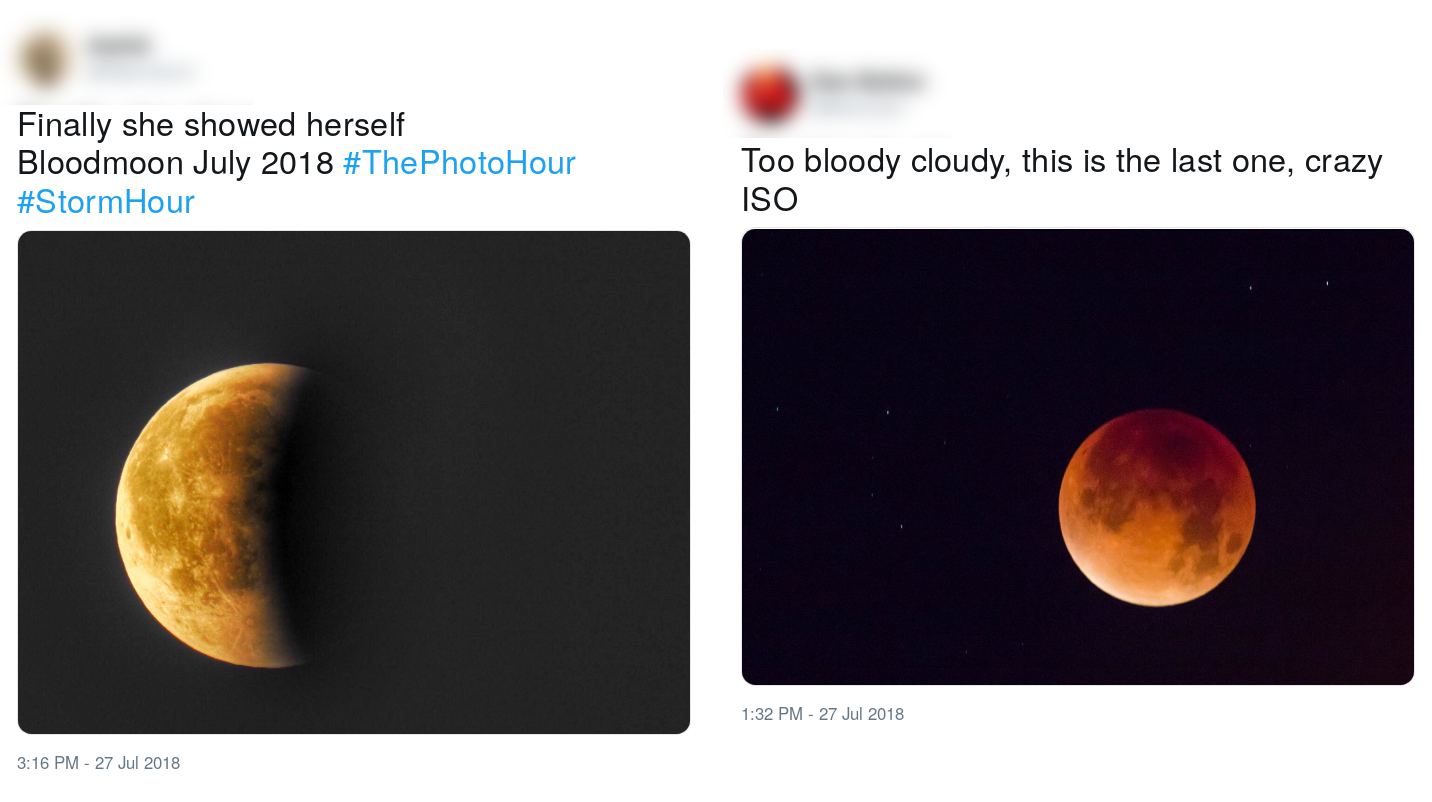
\includegraphics[width=\textwidth]{figures/Moon_horizontal.png}
    \caption{Example of a topic (the July 2018 lunar eclipse) where multimedia contents provide a critical information for topic detection}
    \label{fig:moon}
\end{figure*}
 
 Regarding images, recent progress in the field of visual content description due to deep neural networks provides new ways of representing social media documents by including rich visual features. There are cases where image provides decisive information for event detection (see Fig. \ref{fig:moon}). However, dealing with image tweets often requires a contextual knowledge external to the document. Without this knowledge, image can become a source of error for event detection algorithms compared to text alone.
 



\section{State of the art}

\section{Algorithms}

\section{Text-only approaches}

\section{Multimodal approaches}